\documentclass[conference]{IEEEtran}
\IEEEoverridecommandlockouts
% The preceding line is only needed to identify funding in the first footnote. If that is unneeded, please comment it out.
\usepackage{cite}
\usepackage{amsmath,amssymb,amsfonts}
\usepackage{algorithmic}
\usepackage{graphicx, verbatim}
\usepackage{textcomp}
\usepackage{graphicx}
\usepackage{placeins}
\usepackage{xcolor}
\usepackage[utf8]{inputenc}
\usepackage{listings}
\usepackage{tikz}

\definecolor{codegreen}{rgb}{0,0.5,0}
\definecolor{codegray}{rgb}{0.5,0.5,0.5}
\definecolor{codepurple}{rgb}{0.5,0,0.8}
\definecolor{backcolour}{rgb}{0.99,0.99,0.99}
\lstdefinestyle{mystyle}{
    backgroundcolor=\color{backcolour},   
    commentstyle=\color{codegreen},
    keywordstyle=\color{magenta},
    numberstyle=\tiny\color{codegray},
    stringstyle=\color{codepurple},
    basicstyle=\ttfamily\footnotesize,
    breakatwhitespace=false,         
    breaklines=true,                 
    captionpos=b,                    
    keepspaces=true,                 
    numbers=left,                    
    numbersep=5pt,                  
    showspaces=false,                
    showstringspaces=false,
    showtabs=false,                  
    tabsize=2
}
 
\lstset{style=mystyle}
\def\BibTeX{{\rm B\kern-.05em{\sc i\kern-.025em b}\kern-.08em
    T\kern-.1667em\lower.7ex\hbox{E}\kern-.125emX}}
    
\begin{document}

\title{Ceng435 Term Project Part-2 Report\\
}

\author{\IEEEauthorblockN{Zeynep Erdoğan}
2171577 \\ 
\and
\IEEEauthorblockN{Ayşenur Bülbül}
2171403
}

\maketitle


\section{Introduction}
In this part of the project we constructed a UDP based Reliable Data Transfer protocol with multi-homing and pipelining. 

We were expected to conduct two experiments. Experiment 1 is sending a large file from source to destination using the shortest path we found in Term Project Part 1. We should send this file without losing a packet. We found the shortest path as source-r3-destination before. Thus we used this path for Experiment 1. Experiment 2 is sending the same large file using the others routers. We should send this file, again, without losing a packet and we should transfer some packets through r2 and some through r3. Also, we need to consider if there is any failure in links.

UDP(User Datagram Protocol) is a connectionless protocol. Packets may be lost during transportation. This is why we need some other implementations to ensure reliable transfer. We used selective repeat as our pipeline protocol.


We used Python as our programming language. We create sockets with 
We created sockets with Python using $AF\_INET$, which indicates an Internet protocol version 4 family and $SOCK\_DGRAM$ which indicates a datagram based socket application. Sockets are created in Python with this code:
\begin{align*}
    server = socket(AF\_INET, SOCK\_DGRAM)
\end{align*}

We used $recvfrom()$ function for receiving from server that we bind to the server's port and receiver IP. Also, we used $sendto()$ function to send the input data and acknowledge message.

We implemented a UDP based reliable data transfer protocol for two experiments. For each experiment, we run one script at each node. We take a large file at node $s$ and we created an output file at node $d$ with the data we sent from $s$.

\section{Design of the Project}
We are given a network which has a topology as specified below.
\begin{figure}[h!]
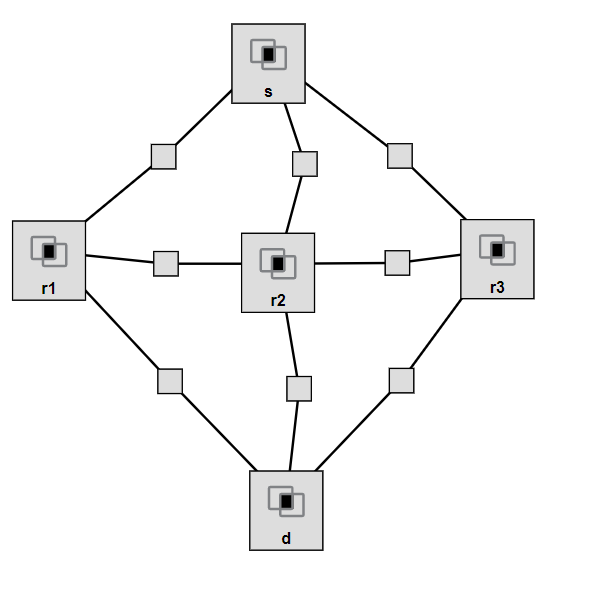
\includegraphics[scale = 0.75]{tp.png}
\caption{Topology of the given network}
\end{figure}
We don't use the links between  r1 and r2, r2 and r3 as asked. For the experiment one we sent the large file through s-r3-d path. For the experiment two, we sent the large file's packets through s-r1-d or s-r2-d depending of the situation(up or down) of the links. If both of the links are up we sent some of the packets from r1 and the other ones from r2.

We designed each packet content as: packet number, checksum result and data. We sent packets with these information from source and we resolved these packets at destination node to send acknowledge back.


\section{Implementation of the Project} 

We have implemented a UDP-based "Reliable Data Transfer" (RDT) protocol of our own that supports selective repeat pipelining and multi-homing. \\
For pipelining we used selective repeat. In selective repeat, receiver acknowledges correctly received packets. Sender waits for a message from receiver that indicates whether or not packet sent to receiver correctly. Sender waits for these messages for a period of time. If timeouts and there is no acknowledged message sent from receiver, sender send this packet again. The difference from go-back-n sender is, in selective repeat, only the non-acked packets are sent again, not the n consecutive ones after the non-acked packet.


For selective repeating, we have an array which we are putting received acknowledge messages for each packet. We first initialized that array with 0 meaning non of the packet is acknowledged. We are keeping our window location as the first not acknowledged packet number. Our sender window length is 100. It sends all 100 messages first and then it times out and sets the window location as the first not acknowledged packets which means if we have received acknowledged for all the packet send then it starts sending next 100 packets but if some packets are lost along the way, It first send those messages. This way packets may not be sent in the correct order at the end but we are putting them order depending on their packet number. \\

We applied multi-homing for experiment 2. Multi-homing is connecting a host to more than one link/network. With multi-homing, the main purpose that we want to achieve is increasing reliability and performance. For this, we sent the large file through both link r1 and r2. We divided the input file into packets. We created two threads, one for sending through r1 and one for sending through r2. For both of these links, we had one $position$ and $windowLocation$ parameters. These parameters are for locating the window's beginning. We used them for data array's index. In that data array we stored packets. We then send packets. If a packet sent from one link, lets say through r1, we don't send it through r2 also. Of course, this case is valid only if both of the links are up. In case of a failure in a link, packets are sent through the link that is still up. We tried and confirmed this by using 
\begin{align*}
    ip \ \ link \ \ set \ \ dev \ \ <interface> \ \ down
\end{align*}
command and set the links down. The data still get sent from the working link.

The overall idea behind the implementation of experiment 1 is explained here: Firstly, source node takes the large input.txt file, divides it into 6250 fragments, each of them size 800 bytes. Thus we have 6250 packets. We calculated each data fragments' checksum using $checksum$ function. This function sets a $result$ variable to 0, takes the data fragment and for each character in it, adds the integer representation of that character(we found this representation using Python's $ord$ function) to the $result$ variable. Then returns the complement of the $result$ variable.  We designed packets with using packet number, checksum result and data. We concatenate packet number, checksum of the data fragment and data fragment with '*-*' character between them. Later on destination node we used this character to separate the message that is sent by source. 

We have two functions in ex1source.py file, $sender$ and $receiver$. $sender$ sends the packets to router r3. To stop the threads, we used an array $acks$. This array every element is 0. $receiver$ function set the elements 1, using the packet numbers as index. At the start of the $sender$ function we check whether the sum of all elements in the $acks$ array equals to 6250. This condition means we get acknowledged message for every packet we sent. This way we ensure all packets received from destination. In $sender$ function we check the position of window and make sure it's not bigger than 6250. Also, we check distance between the start and end position of window does not exceed the window size.
Lastly, we checked through $acks$ array whether that packet is sent before and acknowledged. If these conditions are satisfied we send the packet to the router r3.\\

$receiver$ function in ex1source.py file, receives acknowledged messages from router r3. We also check if the sum of the $acks$ array is equal to 6250. If it is, we stop the threads. In here, we check the non-acknowledged messages using $acks$ array. First we wait for the feedback. Then find the first not acknowledged packet number. If that is equals to packet number comes from feedback that means until that packet all the packets are send successfully, no packet is lost so we set window location to next not acknowledged packet number. If it wasn't equal then we wait for timer to timeout and send lost packets again.\\

We also have $timer$ function which is responsible for timeout. In timer we use $sleep(1.5)$ to set timeout value as 1.5. After that time, if source doesn't received acknowledged message, it sends that packet again.

source sends the packets to r3 using only one thread. While declaring this thread, we gave it an argument, 2, as it would uses r3's IP and route from IP and router tables that we assigned before, while binding sockets. We found these values through GENI platform. 
\begin{lstlisting}[
    basicstyle=\small
]
senderR3 = Thread(target=sender, args=([2]))
receiverR3 = Thread(target=receiver, args=([2]))
timerR3 = Thread(target=timer, args=([2]))
\end{lstlisting}

We used r3 as only a router and run r3new.py file. It takes the message from source and sends it to the destination. Also, it takes the acknowledged message from destination and sends back  to source. We achieved this with defining two function. One is $r3sender$ to transferring data from source to destination. The other is $r3receiver$ for ACK messages from destination to source.  We used two threads for this. One is for $r3sender$ and one is for $r3receiver$. 
\begin{lstlisting}[
    basicstyle=\small
]
t1 = Thread(target=r3sender, args=())
t12 = Thread(target=r3receiver, args=())
\end{lstlisting}

Finally, at destination, we created one fuction $dest$. This function waits message from router r3. If it gets any message, firstly it resolves it using '*-*' character that we added to the message before sending from source. We get the packet number, checksum value and data. Then we calculated the checksum of received data using the same function in the source. Then we checked if the checksum we received from the message is same with the checksum we calculated from the data we received. If they are the same, this means data is sent without being corrupted. Otherwise, data is corrupted so destination does not send acknowledged message to source through destination. We sent empty string if we get corrupted data. Otherwise, we sent packet number to source. We used this as ACK message. We used one thread in destination port, just to get message and send acknowledged message.
\begin{lstlisting}[
    basicstyle=\small
]
t3 = Thread(target=dest, args=([2]))
\end{lstlisting}


The overall idea behind the implementation of experiment 2 is explained here: Firstly, source node takes the large input.txt file again and like in the experiment one it divides and sends the data. Different from experiment one, here we have two routers, r1 and r2. We used one $pos$ and $windowLocation$ and sends each packet only from one link to routers. The other parts are works in the same logic with experiment one. We have 5 threads. Two is for $sender$ function to send r1 and r2, two is for $receiver$ function to receive from r1 and r2 and one is for timer which sets the timeout value. 

\begin{lstlisting}[
    basicstyle=\small
]
senderR1 = Thread(target=sender, args=([0]))
senderR2 = Thread(target=sender, args=([1]))
receiverR1 = Thread(target=receiver, args=([0]))
receiverR2 = Thread(target=receiver, args=([1]))
timerR1 = Thread(target=timer, args=([0]))
\end{lstlisting}

We used r1 and r2 as routers only. They take the message from source and send them to destination. They also take acknowledged messages from destination and send them to source. For r1, we defined two functions $r1sender$ and $r1receiver$. We created two threads one is for sender function the other is for receiver function.
\begin{lstlisting}[
    basicstyle=\small
]
t1 = Thread(target=r1sender, args=())
t12 = Thread(target=r1receiver, args=())
\end{lstlisting}
For r2, we defined two functions $r2sender$ and $r2receiver$. We created two threads one is for sender function and the other is for receiver function.
\begin{lstlisting}[
    basicstyle=\small
]
t1 = Thread(target=r2sender, args=())
t12 = Thread(target=r2receiver, args=())
\end{lstlisting}
And finally, on destination node, we resolved the received image in $dest$ function just like in the experiment 1's script. We have two threads, one is for router r1 and the other is for router r2. We take messages from both of these links, using thread we achieved multi-homing and get better performance.
\begin{lstlisting}[
    basicstyle=\small
]
t2 = Thread(target=dest, args=([1]))
t1 = Thread(target=dest, args=([0]))
\end{lstlisting}

For  node s we have 3 main functions which are sender receiver and timer. For sender our main algorithm is 
\begin{lstlisting}[
    basicstyle=\small
]
create a UDP socket.
while there are still packets that are not ack
    check if current packet number in window
        prepare pckt(packet#,checksum,message)
        send pckt to router
        current packet number ++
close socket
\end{lstlisting}
For receiver our main algorithm is 
\begin{lstlisting}[
    basicstyle=\small
]
create a UDP socket.
bind it to server's port
while there are still packets that are not ack
    receive feedback(packet #)
    find first not ack packet #
    mark received feedback(packet #) as ack
    find second not ack packet
    if feedback is equal to 1. not ack pack
        slide windowloc to 2. not ack packet#
close socket
\end{lstlisting}
For timer our main algorithm is 
\begin{lstlisting}[
    basicstyle=\small
]
while there are still packets that are not ack
    sleep for 1.5 sec //timeout
    current packet = windowlocation
\end{lstlisting}

For routers r1,r2 and r3 same algorithm with different ports and ips are running. We have 2 main functions which are sender and receiver. For sender our main algorithm is 
\begin{lstlisting}[
    basicstyle=\small
]
create a UDP socket.
bind it to destination's port
while true
    receive packet from source
    send it to destination
close socket
\end{lstlisting}
For receiver our main algorithm is 
\begin{lstlisting}[
    basicstyle=\small
]
create a UDP socket.
bind it to server's port
while true
    receive packet from destination
    send it to source
close socket
\end{lstlisting}

For destination we have one main function and it's algorithm is 
\begin{lstlisting}[
    basicstyle=\small
]
create a UDP socket.
bind it to router's port
while there are not ack messages
    receive packet from router
    if cheksum is true
        send received packet# as feedback to router
close socket
\end{lstlisting}

\section{Experiment 1}
For experiment 1, we were expected to configure links between s-r3-d and get the file transfer time. We calculated this time in source node. We take the start time at the beginning of the script and at receiver function when we get the 6250 ACKs, which means we sent all the packets successfully, we get the end time and subtract the end time from start time and print it to the terminal. We configured the links for 5\%, 15\%, 38\% packet losses. 
Since our file transfer times are so big we couldn't run the experiments more than 5 times and we find the error 2.4 percent. \\
As seen in the figure 2 as the packet loss increases file transfer time increases. Since it spends time to sends lost packets again.
\begin{figure}[h]
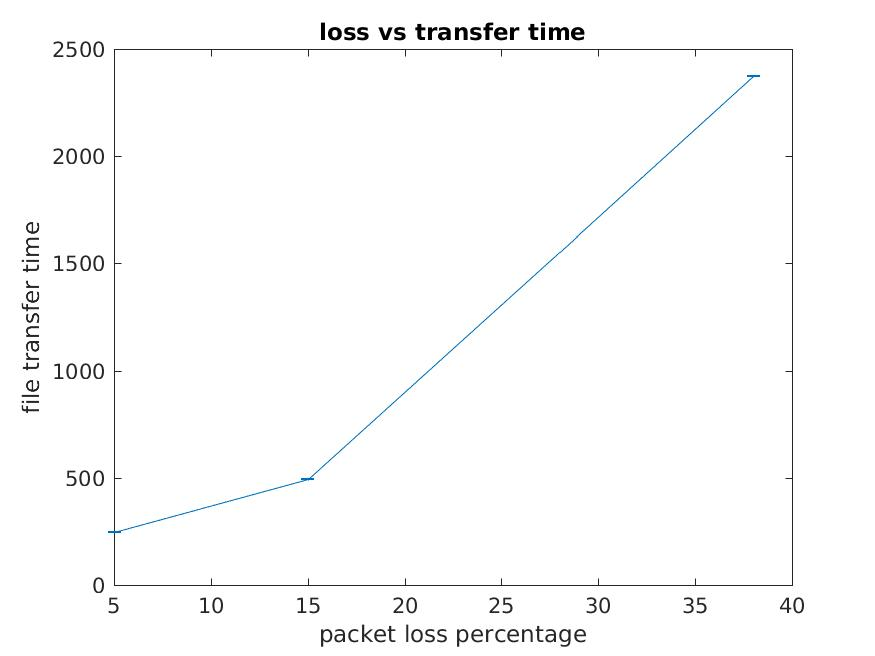
\includegraphics[scale = 0.32]{netpar2ex1.jpg}
\caption{Packet loss percentage vs File transfer time}
\end{figure}
 \FloatBarrier
\section{Experiment 2}
In experiment two there are 2 routes from source to destination. We are expected to apply multihoming which means some of the packets send through router r1 and some routes are send through router r2. Since we have applied selective repeat, order of the packets change in the destination but we put them again to order in destination node depending on their packet number. \\
When we set down one link using the command that we mentioned before on the report, for example link between r1, we get the packets from router r2.
\\
\begin{figure}[h]
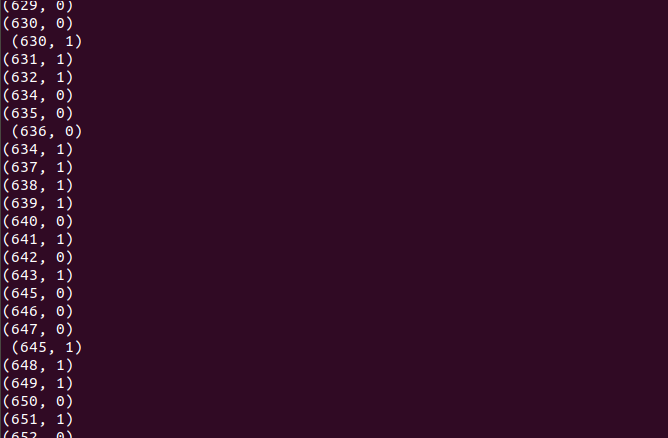
\includegraphics[scale = 0.38]{mh1.png}
\caption{multi-homing 1}
\end{figure}
 \FloatBarrier
 \begin{figure}[h]
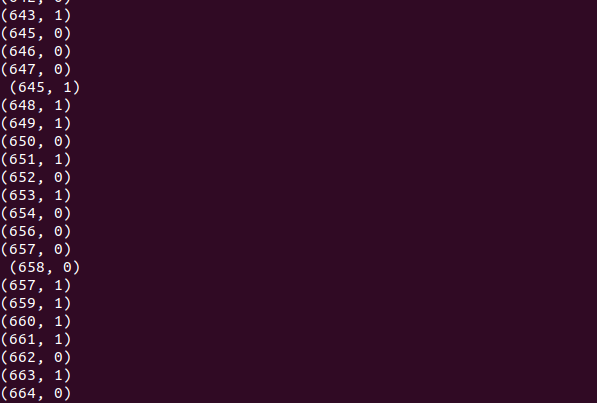
\includegraphics[scale = 0.38]{mh2.png}
\caption{multi-homing 2}
\end{figure}
 \FloatBarrier
  As seen in the figure 3 and figure 4 while sending packets from source to destination in some packets it uses router 1 and in some packets it uses router 2. In figures tuples first element is the packet number and second element is the router number. 0 means router 1 and 1 means router 2.
\begin{figure}[h]
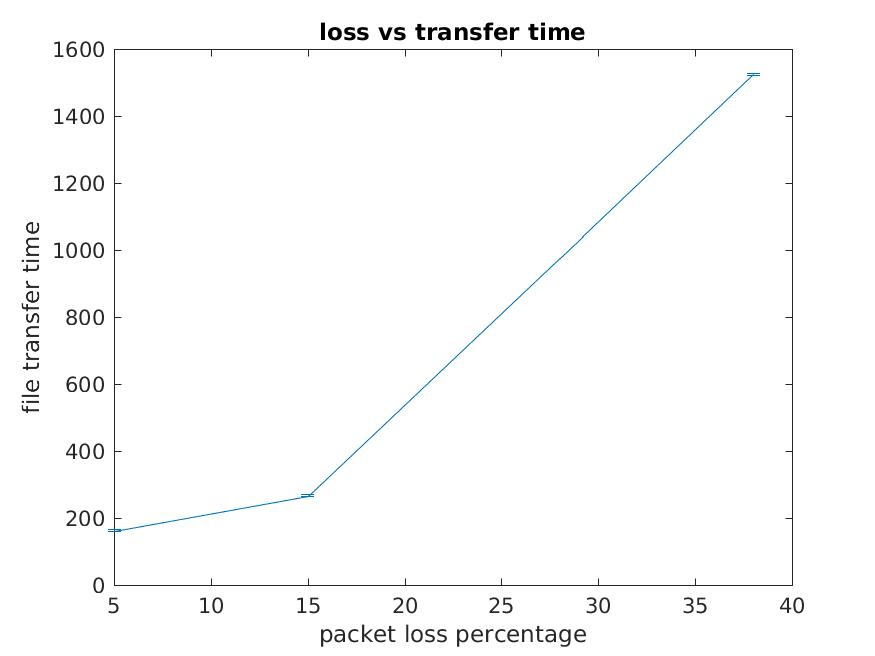
\includegraphics[scale = 0.32]{netpar2ex21.jpg}
\caption{Packet loss percentage vs File transfer time}
\end{figure}
 \FloatBarrier
 Figure 5 shows results of the experiment two. We have done 5 experiment each and find errors similar to experiment one. Comparing to results of the first experiment we can see the decrease in the file transfer time. This is due to multi homing. Instead of sending packets from one route we are sending packets from two routes and balancing the load.
\section{Conclusion}
In this part of the term project We have implemented a UDP-based "Reliable Data Transfer" (RDT) protocol of our own that supports selective repeat pipelining and multi-homing. We have done two experiments. In experiment one since there was only one route from source to destination we didn't implement multi-homing. In experiment two there was 2 route from source to destination. Due to this, results of experiment 1 is bigger than experiment 2. \\
Also in both experiments as the packet loss gets bigger, the file transfer time gets bigger since it spends time to send the packets again. \\
In result of the both experiment we were able to get the same 5 mb text file. \\
We did coding, experimenting and writing the report together.





\end{document}
